\chapter{Implementación}

	\section{El robot bípedo Nimbro OP}
	La implementación de los algoritmos de visión artificial está planeada para usarse para el robot bípedo Nimbro OP (Open Platform) que está diseñado para jugar fútbol, en competencias como la RoboCup \textit{Humanoid League} y es compatible con la categoría \textit{TeenSize}.

	\textit{Nimbro-OP} (Figura \ref{fig:Nimbro-OP}) fue el primer prototipo para modular a los humanoides \textit{open-source} para investigación y educación. 
	\subsubsection*{Características de hardware}
	\begin{itemize}
	\item Cuenta con una altura de 95cm y un peso aproximado de 6.6kg.
	\item 20 actuadores interconectados (motores Dynamixel).
		\begin{itemize}
			\item 6 por cada pierna (MX-106)
			\item 3 por cada brazo (MX-64)
			\item 2 en el cuello (MX-64)
		\end{itemize}
	\item PC con doble núcleo (Zotac ZBOX nano XS)
		\begin{itemize}
		\item Procesador AMD E-450(2x1.65GHz) 
		\item 2GB RAM, 64GB SSD
		\item USB 3.0, HDMI, Gigabit Ethernet
		\end{itemize}
	\item WiFi: IEEE 802.11b/g/n
	\item Cámara de amplio ángulo de visión (Logitech C905)
	\item Sensores de inercia (Dentro del controlador Ronotis CM-730)
		\begin{itemize}
		\item Acelerómetro de 3 ejes
		\item Giroscopio de 3 ejes
		\end{itemize}
	\item Batería de Litio de 11.1V a 4.5Ah
	\item Chasis de fibra de carbono, aluminio y ABS plus
	\end{itemize}
	
	\subsubsection*{características de software}
	\begin{itemize}
	\item El software es compatible tanto para Linux como Windows.
	\item Tiene un desarrollo basado en la plataforma ROS para proporcionar la abstracción de hardware.
	\item Cuenta con software de código abierto que \textit{Robotis} lanzó para DARwin-OP para comportamientos y habilidades básicas en fútbol.
	\end{itemize}
	
\begin{figure}
\centering
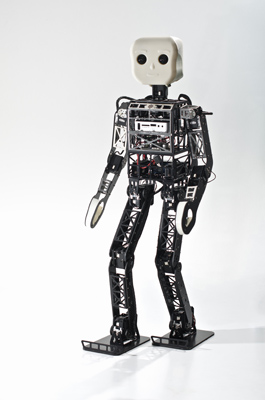
\includegraphics[scale=2.0]{images/Nimbro-OP.jpg}
\caption{Robot humanoide tipo Nimbro-OP}
\label{fig:Nimbro-OP}
\end{figure} 
	
	\section{Las bilbiotecas OpenCV}
OpenCV (\textit{Open Computer Vision}) es una biblioteca \textit{open source} diseñada para visión computacional. Esta biblioteca está escrita principalmente en C y C$++$ y es capaz de ejecutarse en diversos sistemas operativos, tales como: \textit{Windows}, \textit{Linux}, o \textit{Mac OS X}.

OpenCV fue desarrollada para hacer procesos más eficientes cuando se hace visión con aplicaciones en tiempo real. Una de las metas de OpenCV es proveer una infraestructura sencilla y sofisticada para  diferentes tipos de usuarios, que van desde profesores, estudiantes, profesionistas, desarrolladores, y autodidactas. La librería cuenta con más de 500 funciones que se extienden en diversas áreas de visión, incluyendo inspección en la fabricación de productos, seguridad, calibración de cámaras, visión estéreo, robótica, etc.

	Las principales funciones de OpenCV que se utilizaron para la elaboración de este trabajo fueron:  \textit{cv::calibrateCamera()} para hacer la corrección de las distorsiones (véase la sección 3.2), \textit{cv::cvtColor()} para cambiar del espacio de color RGB al HSV, \textit{cv::InRange()} para realizar la segmentación de color del objeto de interés (véase la sección 3.3), \textit{cv::erode()} y \textit{cv::dilate()} para implementar los operadores morfológicos, junto con \textit{cv::findNonZero()} para obtener el centroide de la figura proyectada en la imagen. 
	
	\section{La plataforma ROS}
		\subsection*{¿Qué es ROS?}
Citando a \cite{pyo2015ros} ROS es un meta sistema operativo \textit{open-source} que provee servicios a las aplicaciones de robótica, servicios que comunmente se esperan de un sistema operativo, tales como: abstracción de hardware, control de dispositivos a \textit{bajo nivel}, paso de mensajes entre procesos, ordenamiento y manejo de distintos tipos de paquetes. ROS también provee herramientas y bibliotecas para obtener, construir, escribir y ejecutar programas a través de multiples computadoras.\\

ROS es la abreviación en inglés de \textit{Robot Operating System} lo cual se prodría traducir al español como Sistema Operativo de Robots. Se podría pensar que ROS es un sistema operativo, sin embargo el término mejor empleado es el de \textit{Meta Sistema Operativo}, y aunque no está definido en el diccionario, se puede describir como un sistema que realiza procesos tales como programación, ejecución, monitoreo, y manejo de errores, utilizando una capa de visualización entre aplicaciones y recursos informáticos distribuidos.\\

Dicho lo anterior, ROS no es un sistema operativo convencional, tal como \textit{Windows}, \textit{Linux}, o \textit{Android}, sino una plataforma que se ejecuta dentro del sistema operativo instalado. A menudo, para utilizar ROS se requiere tener instalado \textit{Ubuntu}, que es un sitema basado en las distribuciones de \textit{Linux}. No obstante, es posible usarse en distintos sitemas, tal y como se muestra la figura \ref{fig:meta_operating_system}. 
\begin{figure}
\centering
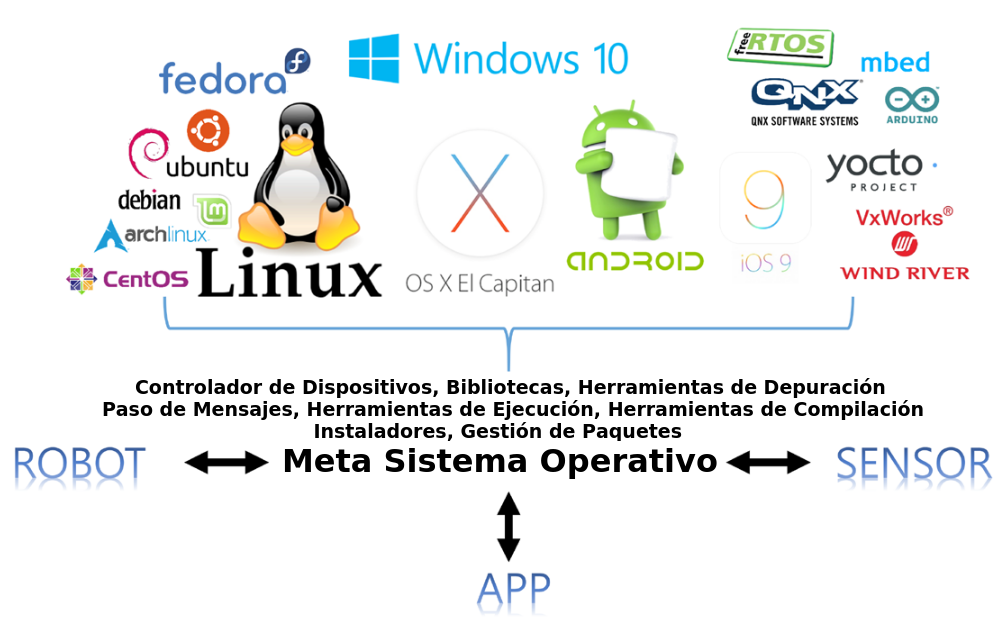
\includegraphics[scale=0.5]{images/meta_operating_system.png}
\caption{Esquema de la abstracción de harware por ROS en distintos Systemas Operativos}
\label{fig:meta_operating_system}
\end{figure} 

		\subsection*{Objetivos al utilizar ROS}
Aunque existen diversas plataformas de robótica (OpenRTM, OPRoS, Player, Orca, Microsoft Robotics Studio, etc.), ROS está orientado a construir entornos de desarrollo para software de robótica a un nivel global, con esto se espera que el código de diferentes desarrolladores se pueda usar, modificar o mejorar para hacer crecer el entorno mismo, es por eso que posee las siguientes características:

\begin{itemize}
\item \textbf{Distribución de procesos:}
Están programados en unidades mínimas de procesamiento (nodos). Cada uno de estos procesos se ejecuta de manera independiente y es capaz de intercambiar datos con otros de manera sistemática.  
\item \textbf{Manejo de paqueterías:}
Cuando varios procesos tienen propósitos similares, estos se manejan dentro de un \textit{paquete} que haga los procesos más ordenados y fáciles de desarrollar.
\item \textbf{Repositorios públicos:}
Cada paquete se hace público dentro de un repositorio (por ejemplo GitHub) para que la comunidad de desarrolladores puedan acceder a él. 
\item \textbf{API (Interfaz de Programación de Aplicaciones):}
Cuando se desarrolla un programa en ROS, generalmente se llaman funciones ya existentes fácilmente insertarlas dentro del código que se esté construyendo.
\item \textbf{Soporte de distintos lenguajes de programación:}
La plataforma ROS posee una \textit{bilioteca de clientes} para facilitar el trabajo de los programadores. La biblioteca puede importar lenguajes de programación que son bastantes populares, tales como Python, C$++$, Java, Ruby, Lips, entre otros.
\end{itemize}
		\subsection*{Breve historia de ROS}
\textit{Robot Operating System} fue creado en Mayo del 2007 dentro del \textit{Standford Artificial Intelligence Laboratory}. Se podría decir que el predecesor de ROS es un proyecto llamado \textit{SwitchYard}, el cual es un software creado para el desarrollo de inteligencia artificial de robots.

En noviembre del 2007 la compañía estadounidense \textit{Willow Garage} empezó el desarrollo de ROS dentro del campo de los robots de servicio. De esta manera ROS vino al mundo oficialmente el 22 de Enero del 2010 con la versión llamada \textit{ROS 1.0}, sin embargo la versión más conocida fue \textit{Box Turtle} lanzada en Marzo del mismo año.

La plataforma ROS es actualizada cada dos años (entre el lapso de Abril-Octubre), lo que significa que cada versión tiene soporte durante aproximadamente cinco años. Para propósitos de esta tesis se optó por utilizar la versión \textit{ROS-Kinetic} instalado en Ubuntu 16.04 \textit{Xenial Xerus (LTS)}.

	\section{Integración de los diferentes programas}
	Para hacer uso del humanoide se requiere clonar un repositorio que se encuentra en la siguiente liga: https://github.com/mnegretev/Humanoids . Este repositorio contiene distintos programas, unos para que el hardware del humanoide se pueda comunicar con un ordenador, otros para el procesamiento de datos, concernientes a las entradas de sensores y control de actuadores e incluso para hacer pruebas remotas con el simulador.
	
	Debido a las circunstancias extraordinarias dadas por la pandemia del coronavirus, el distanciamiento social dificultó la realización de pruebas con el robot físico, por lo que se optó por seguir el desarrollo de software de la parte simulada. Haciendo el software los suficientemente robusto para que sea capaz de usarse tanto en el robot real como en el simulado.
	
	Aunque actualmente no se puedan hacer pruebas con el robot en físico, trabajar con la parte simulada del humanoide representa claras ventajas, las cuales son: 
	 
	\begin{itemize}
	 	\item Complementar el simulador con plug-ins y herramientas extra para la simulación de una cámara virtual dentro del simulador Gazebo.
	 	\item Control del ruido inherente a la medición de los sistemas, ya que se puede probar la robustez del algoritmo de filtrado con diferentes niveles de ruido.
	 	\item Desarrollo del código para el simulador, para su aprendizaje y complementación de la documentación.
	 	\item Hacer el software más disponible para desarrolladores que no tengan la posibilidad de interactuar con el robot o que se encuentren en lugares distantes.
	 	\item Evitar retrazos por fallas del hardware.
	\end{itemize}
	
		\subsection*{Descripción de los principales nodos usados en este trabajo}
		El repositorio anteriormente mencionado tiene instrucciones para la instalación del entorno de trabajo y corrimento de los programas. Para probar el simulador, el comando de inicio es  \textit{roslaunch $surge_-et_-ambula$ $humanoid_-simul.launch$} el cual es un comando que levanta distintos nodos que se comunican entre sí para simular las variables físicas del robot. 
		
		Cuando se levanta se puede observar que se abren algunas ventanas, las cuales son del visualizador del robot \textit{Rviz}, el simulador con variables físicas \textit{Gazebo}, una GUI (Graphical User Interface) para manipular las articulaciones del robot y una ventana que simula la imagen obtenida de la cámara simulada. Tal y como se observa en la Figura \ref{fig:gazebo}.
		
\begin{figure}
	\centering
	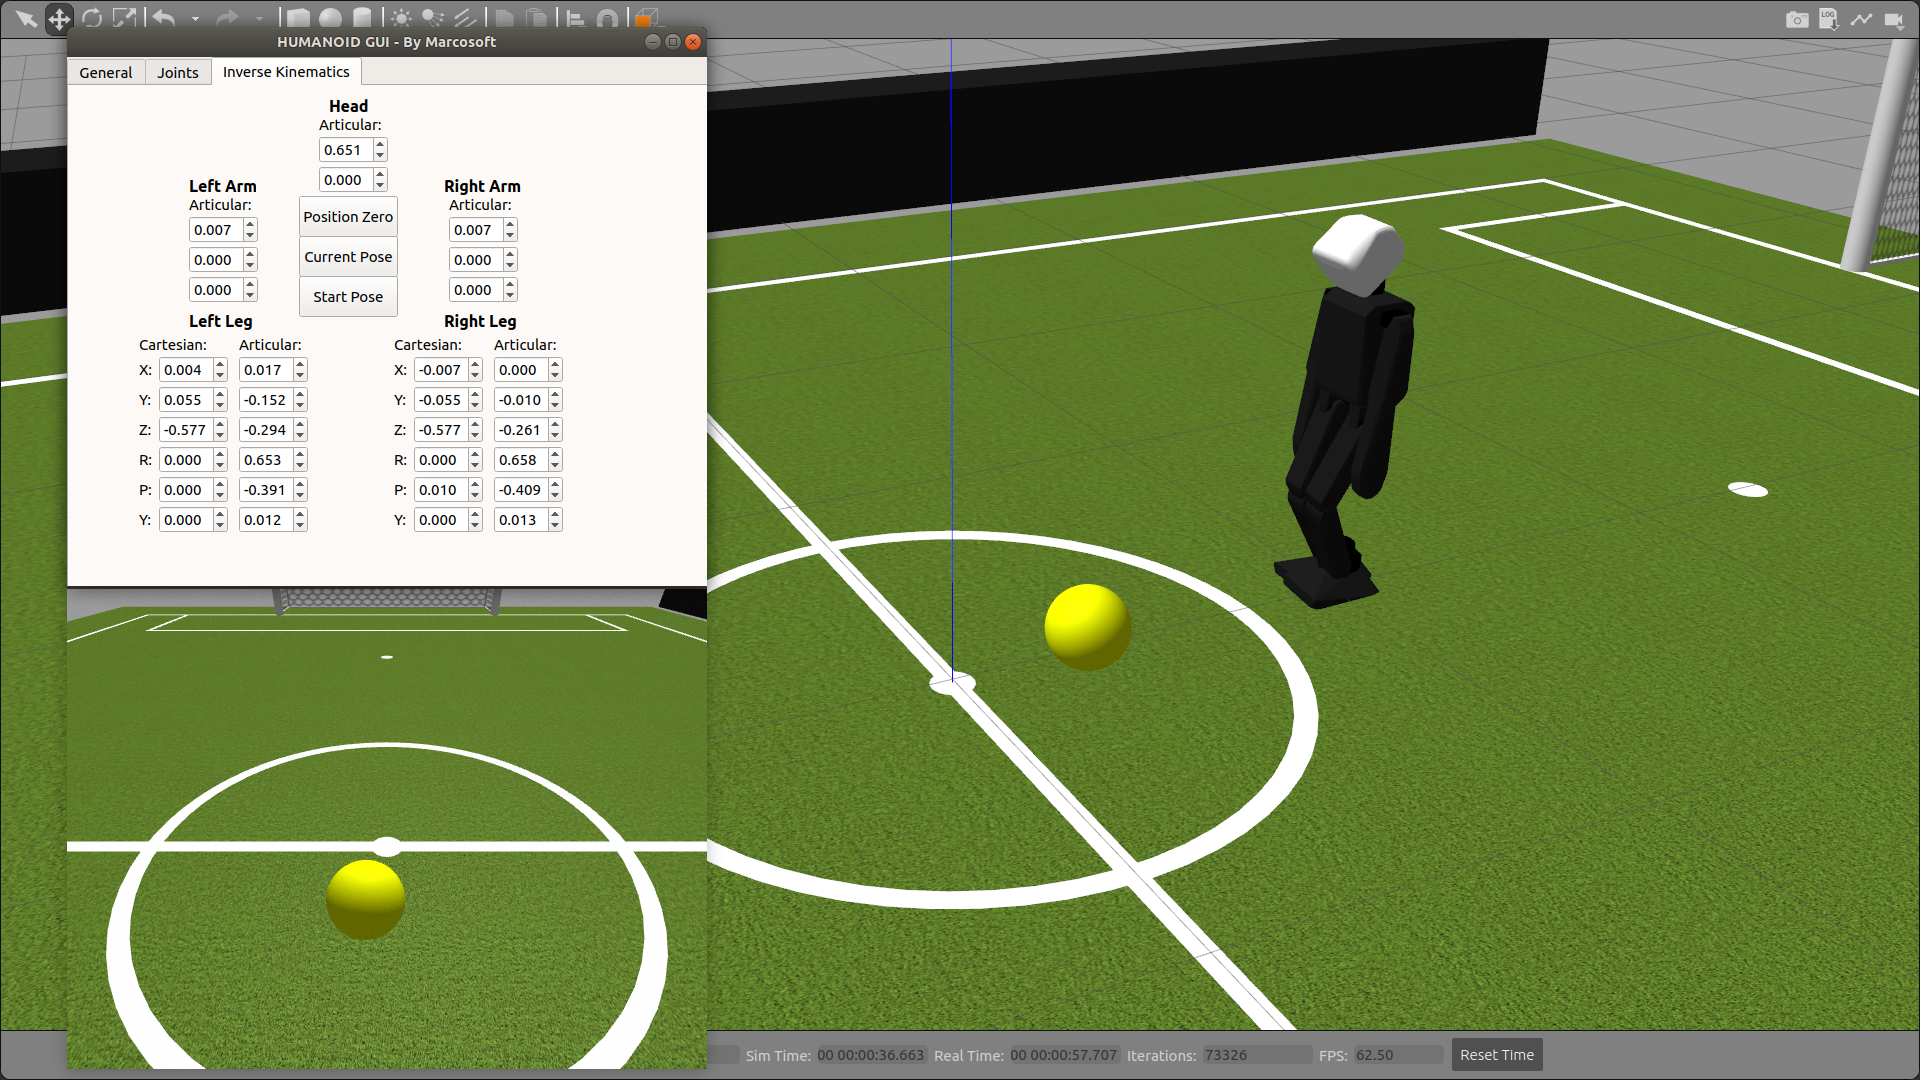
\includegraphics[scale=0.2]{images/gazebo.png}
	\caption{Simulador Gazebo para el humanoide.}
	\label{fig:gazebo}
\end{figure} 
		
			\subsubsection*{Nodo segmentador de color}
			Ejecutano el comando \textit{rosrun $ball_-tracker$ $ball_-tracker_-simul$} se alza el nodo que se subscribe a los tópicos que contienen la información de la imagen RGB obtenida por la cámara. Con esa información se procesa la imagen para segmentar un color deseado guardando los parámetro HSV en un archivo .xml.
			
			\subsubsection*{Nodo que calcula la posición relativa del balón}
			El nodo más importante de esta tesis es el que calcula la posición relativa del balón, ya que de éste depende la precisión y confiabilidad de las mediciones. Con el comando \textit{rosrun $ball_-position$ $ball_-position_-simul$} se levanta, se subscribe a los tópicos de la imagen y hace la segmentación del objeto de interés con base en la teoría vista en el capítulo 3. 
			
			Teniendo ya procesada la sementación, el punto de interés de la figura segmentada es el centroide, con el cual se hacen cálculos geométricos para el posicionamiento del balón, haciendo uso de las herramientas \textit{tf} para conocer la posición y orientación relativa de la cámara con respecto a los pies del robot. Como se ilustra en la Figura \ref{fig:tf}.
			
\begin{figure}
	\centering
	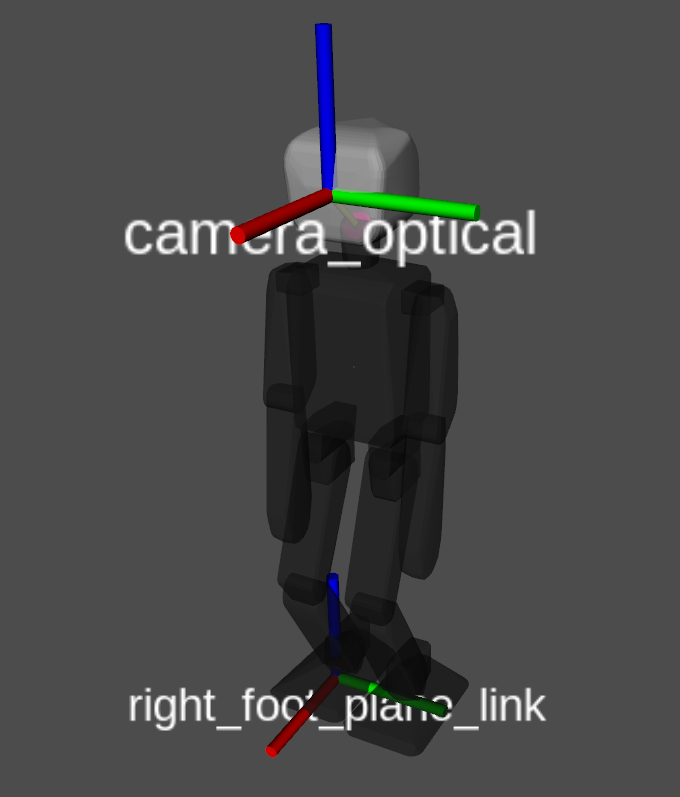
\includegraphics[scale=0.2]{images/tf.png}
	\caption{tf, herramienta de ROS para obtener la información relativa de las articulaciones de un robot (posición y orientación)}
	\label{fig:tf}
\end{figure}
	
			Al procesar la información de posición, el nodo $ball_-position_-simul$ publica un tópico que contiene la posición $X$ y $Y$ del balón, por lo que otros nodos pueden hacer uso de esa información. El código de este nodo puede verse en el Apéndice A.
			
			\subsubsection*{Nodo estimador de posición y velocidad utilizando el Filtro de Kalman Extendido}
			El nodo llamado $kalman_-estimator$ es un \textit{script} escrito en el lenguaje Python, el cual se subscribe a los tópicos de posición del balón y hace una comparación entre ellos para obtener su velocidad instantánea. Con esto, el programa usa los parámetros de Kalman (véase la sección 4.3) para obtener una correción del ruido y su debida predicción de posiciones tomando una determinada cantidad de muestras con una frecuecia aproximada de 30 Hz. El código de este nodo puede verse en el Apéndice B.
			
			\subsubsection*{Nodo para movimiento del balón}
			Ejecutando en una nueva terminal el comando \textit{rosrun $ball_-position$ $move_-ball_-node$ 2.5} se inicializa un nodo que mueve el balón simulado a una dirección y velocidad inicial determinada, con base el lo que se vio en la sección 4.2. 
			
			\subsubsection*{Nodo para la secuencia de pateo} 
			El programa que ejecuta el nodo \textit{$ready_-2_-kick$} utiliza la clase Humanoid para hacer movimientos con posiciones predefinidas, en este caso pausandolas para mantenerse parado sobre un pie esperando a que el nodo $kalman_-estimator$ le de la señal para que patee el balón.
		
		
		
		
		
		
		
		
		
		
		